\documentclass[a4paper, 12pt]{article}

\usepackage[portuguese]{babel}
\usepackage{blindtext}
\usepackage{mathptmx}
\usepackage{microtype}
\usepackage{enumitem}
\usepackage{amsmath}
\usepackage{index}
\usepackage{fancyhdr}
\usepackage{tikz}
\usepackage{amssymb}
\usepackage{float}
\usepackage{nicematrix}
\usepackage{xcolor}
\usepackage{soulutf8}
\usepackage[hyphens]{url}
\usetikzlibrary{matrix}
\usetikzlibrary{patterns,decorations.pathreplacing}
\usepackage{graphicx}
\graphicspath{ {./} }

\DeclareUnicodeCharacter{2212}{-}
\newcommand*\circled[1]{\tikz[baseline=(char.base)]{
            \node[shape=circle,draw,inner sep=2pt] (char) {#1};}}
\newcommand*\R{\mathbb{R}}
\newcolumntype{C}{>{\centering\let\newline\\\arraybackslash\ $}m{0.12cm}<{$}}


\begin{document}
\title{\Large{\textbf{Projeto 2}}}
\author{
\begin{tabular}{c r}
Gabriel Belém Barbosa&RA: 234672\\
Diogo Batalha&RA: 169955\\
Felipe Kenzo Obata Piton&RA: 171108\\
Felipe Purini Policastro&RA: 215760\\
\end{tabular}
}
\date{22 de Maio de 2021}

\maketitle
\let\cleardoublepage\clearpage
\newpage
\setcounter{page}{2}
\tableofcontents
\newpage

\section{Introdução}
O problema de quadrados mínimos (QM) lineares é de fundamental importância em diversas áreas do conhecimento, como nas engenharias e na física experimental e computacional, entre outras. O porblema baseia-se em encontrar, através de equações lineares, uma curva ou superfície em maiores dimensões que melhor se adequa a pontos de interesse. Mais especificamente, busca-se obter
\[
\underset{x\in \R^n}{min}\frac{1}{2}||Ax − b||_2^2
\]
em que $A \in R^{m\times n}$ e $b \in \R^m$. Encontrar $x$ que satisfaz a equação acima é o mesmo que resolver o sistema $A^TAx=A^Tb^{[1]}$, denominado sistema normal.

Solucionar tal sistema é um objetivo que aparece na obtenção de alternativas computacionalmente econômicas para conferir valores de uma função de interesse em um dado intervalo, ou para a melhor visualização, entendimento do comportamento ou confirmação da teoria por trás de dados experimentais. Utilizando um sistema algébrico matricial, esse projeto busca analisar métodos numéricos para a simplificação do sistema normal, no qual fundamenta-se a solução de quadrados mínimos.

Mais objetivamente, a Parte I desse projeto visa a análise qualitativa e de custo de formas do tratamento de um problema teste e seu respectivo sistema normal, nominalmente a solução de equações normais via fatoração de Cholesky, solução via decomposição $QR$ condensada através do processo de Gram-Schmidt modificado (GSM) e fatoração $QR$ completa com transformações de Householder. Além disso, na Parte II, munido das conclusões obtidas dos resultados anteriores, um novo problema será apresendo e tratado com a escolha justificada de um dos três métodos.
\section{Desenvolvimento}
\subsection{Parte I. Comparando diferentes abordagens.}
\subsubsection{Problema teste}
O sistema algébrico matricial escolhido foi \verb+Octave+. Com o intuito de aproximar numericamente a curva de $f(x)=exp(sen(6x))$ em $x\in[0,1]$, usa-se a função \verb+linspace+ do \verb+Octave+ para obter-se o espaço de $x$, \verb+Xspace+, com 21 elementos igualmente espaçados no intervalo desejado. Após isso é construída a matriz de Vandermonde desse espaço de $x$  usando a função \verb+vander+. Esta é da forma
\[
\begin{pmatrix}
x_0^{20}&x_0^{19}&\hdots&x_0^0\\
x_1^{20}&x_1^{19}&\hdots&x_1^0\\
\vdots \\
x_{20}^{20}&x_{20}^{19}&\hdots&x_{20}^0
\end{pmatrix}
\]
Porém, como se deseja um polinômio de grau 10 somente, eliminam-se as primeiras 10 colunas dessa matriz. Também é obtido o espaço associado ao espaço em $x$, \verb+Yspace+, aplicando $f(x)$ ponto a ponto. O sistema linear para o qual deseja-se encontrar a solução de quadrados mínimos fica
\[
\underbrace{
\begin{pmatrix}
x_0^{10}&x_0^9&\hdots&x_0^0\\
x_1^{10}&x_1^9&\hdots&x_1^0\\
\vdots \\
x_{20}^{10}&x_{20}^9&\hdots&x_{20}^0
\end{pmatrix}}_A
\underbrace{
\begin{pmatrix}
c_{10}\\
c_9\\
\vdots \\
c_0
\end{pmatrix}}_c
\simeq
\underbrace{
\begin{pmatrix}
y(x_0)\\
y(x_1)\\
\vdots \\
y(x_{20})
\end{pmatrix}}_y
\]
Em que $c$ a matriz dos coeficientes desejada. A matriz $A$ resultante é uma matriz  $m\times n$ com $m>n$ e posto completo $n$, e o problema recai no sistema normal $A^TAc=A^Ty$, sendo a aplicação de uma fatoração $QR$ de $A$, $Q$ matriz ortogonal e $R$ triangular superior, empregada para que a solução seja
\begin{align}
\label{eqn:nor}
c&=(A^TA)^{-1}A^Ty \nonumber \\
&=(R^TQ^TQR)^{-1}R^TQ^Ty \nonumber \\
&=(R^TR)^{-1}R^TQ^Ty \nonumber \\
&=R^{-1}(R^T)^{-1}R^TQ^Ty \nonumber \\
&=R^{-1}Q^Ty
\end{align}
Onde foi usado que $R$ é invertível e $Q$ ortogonal por construção. Ao contrário de uma decomposição algébrica de $A$, o que é obtido em qualquer método numérico, na realidade, são aproximações $\tilde{R}$ e $\tilde{Q}$ tal que $A=\tilde{Q}\tilde{R}+E$, sendo $E$ uma correção para os erros numéricos. De fato, sequer a matriz $\tilde{Q}$ é ortogonal, sendo, no entanto, possivelmente próxima de o ser numericamente, dependendo da estabilidade do método e do condicionamento da própria matriz $A$. Além disso, há a solução do sistema normal em si, que carrega e intensifica erros e gera novos arredondamentos, independe da fatoração, fato esse que que será tratado na Análise e Discussão ao final desta parte com a separação do erro em estágios. 

Vale notar que as colunas da $A$ poderiam ser permutadas, sabendo-se que a mesma permutação ocorreria entre os elementos de $c$, isto é, ao se permutar as colunas $j$ e $k$ de $A$, ao final do processo o coeficiente $c_j$ e $c_k$ estariam um no lugar do outro em $c$. Tais permutações, entretanto, não afetam o número de condição e a estabilidade do problema, pois, sendo $P$ uma matriz de permutação, e sendo, portanto $P^{-1}=P^T$, tem-se que o número de condição na norma 2, $\kappa_2$, de $PA$ é
\[
\kappa_2(PA)=\frac{\sigma_{max}(PA)}{\sigma_{min}(PA)}=\sqrt{\frac{\lambda_{max}(A^TP^TPA)}{\lambda_{min}(A^TP^TPA)}}=\sqrt{\frac{\lambda_{max}(A^TA)}{\lambda_{min}(A^TA)}}=\frac{\sigma_{max}(A)}{\sigma_{min}(A)}=\kappa_2(A)
\]
Com a notação usual para valores essenciais, $\sigma$, e autovalores, $\lambda$.

\subsubsection{Procedimento}
Para solucionar por transformações de Householder, foi usada a função já presente no \verb+Octave+, \verb+qr+, cuja rotina é baseada em Householder$^{[1]}$. A função aplicada em $A$ já retorna as matrizes $Q_H\in \R^{m\times m}$ e $R_H\in \R^{m\times n}$ em suas formas completas, e o processo demanda teoricamente $2mn^2-\frac{2n^3}{3}-2mn+\frac{2n}{3}\text{ }flops^{[3]}$. Vale ressaltar que a matriz $R_H$ desse processo não é necessariamente equivalente as dos demais métodos (mesmo desconsiderando erros numéricos) devido às escolhas estabilizadoras que não garantem positividade estrita da diagonal principal.
 
Para a fatoração de Cholesky, usa-se a função \verb+chol+, empregada na matriz $A^TA\in \R^{n\times n}$ quadrada positiva definida de posto completo para a obtenção de $R_C\in \R^{n\times n}$ condensada com elementos da diagonal estritamente positivos, esta então sendo usada para a obtenção de $Q_C\in \R^{m\times n}$, também em sua forma condensada, através da solução da relação de matrizes $Q_CR_C=A$, uma vez que a matriz $R_C$ obtida é em teoria a mesma encontrada por GSM de $A^{[2]}$, e portanto possui sua contraparte ortogonal que obedece a relação. O custo operacional de multiplicar $A^TA$ é $2mn^2-n^2 flops^{[5]}$, enquanto o custo de sua fatoração de Cholesky é $\frac{n^3}{3}+\frac{n^2}{2}+\frac{n}{6}\text{ }flops^{[5]}$, e por fim a solução de $Q_CR_C=A$, efetuada como $Q_C=AR_C^{-1}$ demanda $\frac{n^3}{3}+\frac{2n}{3}\text{ }flops^{[5]}$ para a inversão da matriz triangular $R$ e mais $n^3\text{ }flops^{[5]}$ para multiplicação entre a matriz sólida $A\in \R^{m\times n}$ e $R_C^{-1}$, também triangular. O custo total é, em teoria, $2mn^2+\frac{5n^3}{3}-\frac{n^2}{2}+\frac{5n}{6}\text{ }flops$.

Já para GSM, um simples algoritmo foi desenvolvido com base na teoria desse método$^{[2]}$, começando com as matrizes nulas $\R^{n\times n}$ e $\R^{m\times n}$, que serão preenchidas para se tornarem $R_{GS}$ e $Q_{GS}$ respectivamente, ambas na forma condensada, como a seguir.
\begin{verbatim}
Para j=1,2,...,n faça
   Para i=1,2,...,j-1 faça
      r(i,j)=<qi,aj>
      aj=aj-r(i,j)*qi
   r(j,j)=norma2(aj)
   Se r(j,j) é nulo
      Pare
   qj=aj/r(j,j) 
\end{verbatim}
Sendo \verb+ap+ e \verb+qp+ as $p$-ésimas colunas de $A$ e $Q_{GS}$, respectivamente, e o produto interno sendo o usual. Como o posto de $A$ é completo, o algoritmo não para prematuramente. Vale ressaltar que o algoritmo acima destrói a matriz original $A$ durante o processo, portanto uma matriz auxiliar que é uma cópia de $A$ deve ser empregada caso deseja-se trabalhar com esta última após a desomposição. O custo operacional teórico é $2mn^2+mn\text{ }flops^{[4]}$.

Ao final das 3 fatorações é efetuado o comando \verb+c=R\(Q'*Yspace)+ que resolve o sistema normal simplificado, como visto em (\ref{eqn:nor}), encontrando a solução dos coeficientes ótimos. Como esse passo é o mesmo para todos os métodos, ele não agrega nada à análise de custo operacional, e será omitido da contagem de $flops$.

\subsubsection{Análise e discussão}
Os coeficientes encontrados para cada método são apresentados a seguir.
\begin{table}[h]
\centering
\caption{\label{tab:coef} Coeficientes ótimos obtidos por cada método}
\begin{tabular}{|c||c|c|c|}
\hline&Householder&Cholesky&GSM\\
\hline \hline$c_{10}$&2718.7511&2718.6578&2718.7511\\
\hline$c_9$&-11252.3527&-11251.9155&-11252.3528\\
\hline$c_8$&17030.607&17029.7489&17030.6072\\
\hline$c_7$&-8947.7019&-8946.7896&-8947.7022\\
\hline$c_6$&-4124.843&-4125.4097&-4124.8428\\
\hline$c_5$&7503.2788&7503.4845&7503.2787\\
\hline$c_4$&-3523.8442&-3523.8846&-3523.8441\\
\hline$c_3$&622.2207&622.224&622.2207\\
\hline$c_2$&-33.8651&-33.865&-33.8651\\
\hline$c_1$&7.5069&7.5069&7.5069\\
\hline$c_0$&0.99926&0.99926&0.99926\\ \hline
\end{tabular}
\end{table}
\\
Foi obtido também o maior erro pontual entre a aproximação $QR$ e $A$ para cada método, como visto a seguir.
\begin{table}[H]
\centering
\caption{\label{tab:maxdif} Máxima diferença absoluta entre $A$ e $QR$ de cada método}
\begin{tabular}{|c||c|c|c|}
\hline&Householder&Cholesky&GSM\\
\hline \hline max(abs($QR-A$))&1.3323e-15& 2.1538e-10& 3.3307e-16\\ \hline 
\end{tabular}
\end{table}
Com o intuito de separar as influências dos métodos no erro final do polinômio aproximador dos demais processos, foi calculado, para cada método, o erro quadrático médio (MSE-mean squared error) entre a aproximação para $QR$ e $A$ além do MSE entre o polinômio encontrado e sua contraparte $f(x)$ (\verb+Yspace+), como pode ser visto na tabela a seguir. O MSE é calculado como a soma dos quadrados das diferenças ponto a ponto das matrizes ou vetores em questão, dividida pelo número de elementos. Também foram plotadas as diferenças ao quadrado ponto à ponto em função de $x$ para as três abordagens, que estão em três gráficos no Apêndice.
\begin{table}[h]
\centering
\caption{\label{tab:mse} MSE's de cada método}
\begin{tabular}{|c||c|c|c|}
\hline&Householder&Cholesky&GSM\\
\hline \hline MSE($QR,A$)&5.2588e-32&3.9864e-22&3.9640e-33\\
\hline MSE($Ac,f(x_i)$)&1.8062e-05&1.8062e-05&1.8062e-05\\ \hline
\end{tabular}
\end{table}
\\
A tabela a seguir contem o número teórico de $flops$ encontrados anteriormente.
\begin{table}[h]
\centering
\caption{\label{tab:flo} Número teórico de $flops$ por método}
\begin{tabular}{|c||c|c|c|}
\hline&Householder&Cholesky&GSM\\
\hline \hline $flops$&$2mn^2-\frac{2n^3}{3}-2mn+\frac{2n}{3}$&$2mn^2+\frac{5n^3}{3}-\frac{n^2}{2}+\frac{5n}{6}$&$2mn^2+mn$\\ \hline
\end{tabular}
\end{table}
\\
Usando a função \verb+cond+ do \verb+Octave+, cuja rotina envolve a decomposição em valores essenciais$^{[6]}$, foi calculado o número de condição na norma 2, $\kappa_2$, das matrizes triangulares obtidas com cada método, como visto a seguir.
\begin{table}[H]
\centering
\caption{\label{tab:kap} Número de condição de $R$ por método}
\begin{tabular}{|c||c|c|c|}
\hline&Householder&Cholesky&GSM\\
\hline \hline $\kappa_2(R)$&2.3175e+07&2.3126e+07&2.3175e+07\\ \hline
\end{tabular}
\end{table}
E também foi obtido o número de condição $\kappa_2(A^TA)=$5.3699e+14. Apesar do grande número de condição de $A^TA$, a precisão computacional e estabilidade dos três métodos é suficiente para gerar uma boa aproximação de $A$, como visto na Tabela~\ref{tab:mse}, sendo o maior MSE dentre os métodos o da fatoração de Cholesky, na ordem de $10^{-22}$, e o pior erro pontual na Tabela~\ref{tab:maxdif}, também proveniente desse método, é na ordem de $10^{-10}$. Isso implica que, apesar de erros numéricos, e sendo os $\kappa_2$ na Tabela~\ref{tab:kap} na ordem de $10^7$, os erros para a aproximação de $A$ são irrisórios comparados com o que seria necessário para diferenças significativas dado o número de condição do sistema normal $Rc=Q^Ty$, mesmo considerando o elemento de maior imprecisão de qualquer método (é um sistema relativamente bem condicionado dada a precisão de máquina e estabilidade dos métodos). Para o problema em questão, portanto, a Tabela~\ref{tab:flo} é a mais relevante quando se trata de decidir qual dos métodos é o mais adequado, sendo, dentre as opções, a fatoração de Householder a mais econômica e que melhor escala com a ordem do problema.

\subsection{Parte II. Algo mais.}
O problema de quadrados mínimos aparece comumente em aproximação de dados experimentais. Nesse contexto, muitas vezes as funções aproximadoras escolhidas são diversas e vão além de simples polinômios como aquele usado no problema teste, dependendo da natureza dos dados em questão. Para essa parte será apresentado um problema de modelagem de dados de poluição atmosférica na forma da concentração de $NO$  em uma rua movimentada durante um período de 24 horas (veja o exemplo 2 e 3 em [8]). A aproximação será através de funções trigonométricas e uma constante. Os dados experimentais são
\begin{table}[h]
\centering
\caption{\label{tab:no} Concentração de NO $y_i$ ($\mu g/m^3$) em função do tempo $t_i$ (Horas)}
\begin{tabular}{|c r|c r|c r|c r|c r|}
\hline$t_i$ &$y_i$ &$t_i$ &$y_i$ &$t_i$ &$y_i$ &$t_i$ &$y_i$ &$t_i$ &$y_i$\\
\hline 0 &110.49 &5 &29.37 &10 &294.75 &15 &245.04 &20 &216.73\\
1 &73.72 &6 &74.74 &11 &253.78 &16 &286.74 &21 &185.78\\
2 &23.39 &7 &117.02 &12 &250.48 &17 &304.78 &22 &171.19\\
3 &17.11 &8 &298.04 &13 &239.48 &18 &288.76 &23 &171.73\\
4 &20.31 &9 &348.13 &14 &236.52 &19 &247.11 &24 &164.05\\
\hline
\end{tabular}
\\Fonte: Mahooti, 2019
\end{table}
\\
As funções escolhidas para a aproximação de dados são 
\[
f_0(t) = 1, f_1(t) = sin(\omega t), f_2(t) = cos(\omega t), f_3(t) = sin(2\omega t), f_4(t) = cos(2\omega t), ...
\]
Com o total de nove funções, sendo $w=\frac{\pi}{12}$ o fator de correção que transforma o ciclo de 24 horas em $2\pi$, o que é proveitoso para que todas as funções envolvidas, ao término de um dia, se repitam exatamente no próximo, criando um ciclo dário. Haverão 25 equações lineares da forma
\[
y_i = c_0 + c_1sin(\omega t_i) + c_2cos(\omega t_i)+...+ c_8cos(4\omega t_i), i = 0, 1, . . . , 24
\]
O sistema cuja melhor aproximação é buscada fica
\[
\underbrace{
\begin{pmatrix}
cos(4\omega t_0)&sin(4\omega t_0)&\hdots&1\\
cos(4\omega t_1)&sin(4\omega t_1)&\hdots&1\\
\vdots \\
cos(4\omega t_{24})&sin(4\omega t_{24})&\hdots&1
\end{pmatrix}}_A
\underbrace{
\begin{pmatrix}
c_8\\
c_7\\
\vdots \\
c_0
\end{pmatrix}}_c
\simeq
\underbrace{
\begin{pmatrix}
y_0\\
y_1\\
\vdots \\
y_{24}
\end{pmatrix}}_y
\]
Utilizando a função \verb+linspace+, em seguida foi construído o espaço de $t$, \verb+Tspace+, e também montado o espaço \verb+Yspace+ com os valores de $y$ da Tabela~\ref{tab:no}. Através de operações vetoriais do \verb+Octave+ sobre \verb+Tspace+ foi construída a matriz $A$ como descrita. Aqui foi usada a decomposição de Householder e a solução do sistema normal da mesma maneira do problema teste, usando a relação (\ref{eqn:nor}). Este método foi escolhido pelos mesmos motivos citados na Análise e Discussão da Parte I, isto é, o menor custo computacional e equivalente performance dentro das margens de precisão desejadas. Os coeficientes encontrados foram
\begin{table}[h]
\centering
\caption{\label{tab:coef2} Coeficientes ótimos da modelagem de dados atmosféricos}
\begin{tabular}{|c||c|}
\hline&Valores\\
\hline\hline$c_8$&-7.5190\\
\hline$c_7$&    -5.8197\\
\hline$c_6$&    37.3292\\
\hline$c_5$&    25.4682\\
\hline$c_4$&     1.7667\\
\hline$c_3$&   -58.4353\\
\hline$c_2$&   -93.4740\\
\hline$c_1$&   -73.2370\\
\hline$c_0$&   189.2455\\ \hline
\end{tabular}
\end{table}
\\
E a seguir o gráfico do erro ponto a ponto ao quadrado.
\begin{figure}[H]
\centering
\caption{\label{fig:1} Erro quadratico ponto a ponto}
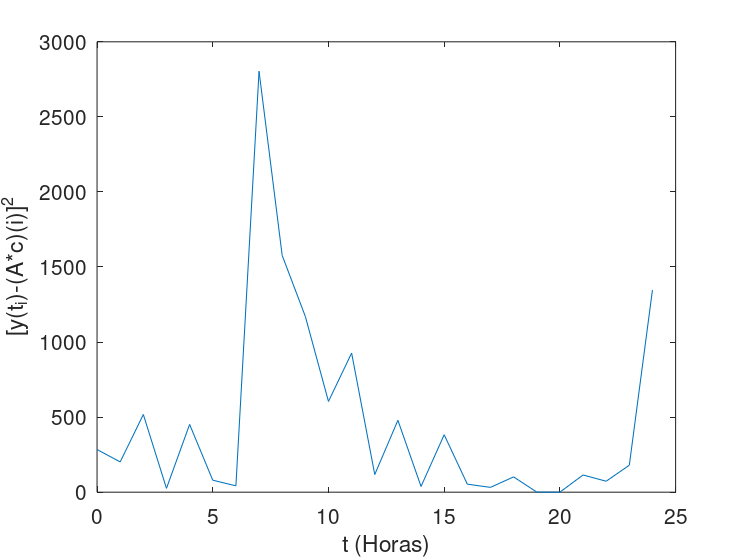
\includegraphics[width=11cm]{err2}
\end{figure}
E o gráfico dos dados e da aproximação sobrepostos.
\begin{figure}[H]
\centering
\caption{\label{fig:2} MMQ vs. $y(t_i)$}
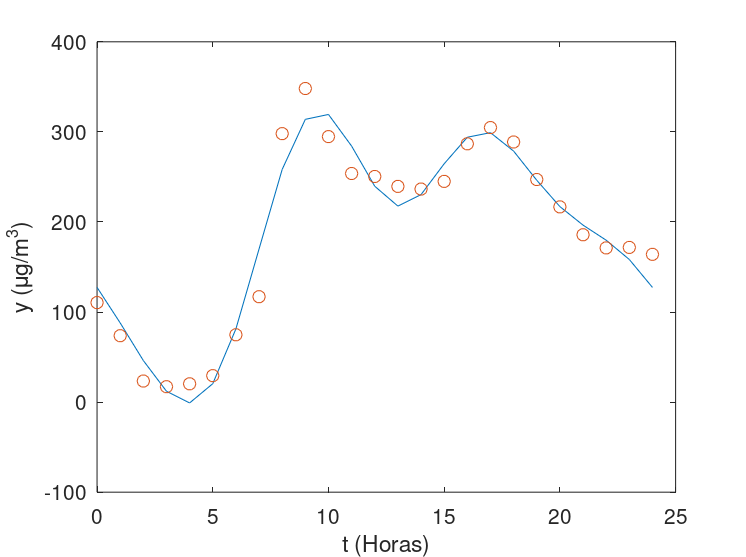
\includegraphics[width=11cm]{MMQ2}
\end{figure}
O MSE entre os pontos experimentais e a aproximação foi de 464.18, o que não é de se surpreender para uma modelagem de dados experimentais (que não seguem precisamente uma função devido ao \textit{white noise}$^{[7]}$) dada a magnitude dos valores envolvidos. O pior erro pontual entre a fatoração $QR$ numérica por Householder e a matriz $A$ original foi de 1.1102e-15, enquanto o MSE entre estes foi de somente 5.0901e-32. O $\kappa_2$ da matriz $R$ encontrada e de $A^TA$ são 1.4556 e 2.1187, respectivamente, sendo então esse problema, em comparação, muito mais estável que o anterior, portanto as mesmas conclusões anteriores (com respeito à análise dos erros dos métodos em contraste aos números de condição) são aplicáveis ao problema atual. 
\section{Conclusão}


\section{Referências}
\begin{enumerate}
\sloppy
\item C. B. Moler, \textit{Numerical Computing with MATLAB}, Philadelphia: SIAM, 2004.
\item D. S. Watkins, \textit{Fundamentals of Matrix Computations}, New Jersey: John Wiley \& Sons, 2 ed., 2002.
\item R. A. van de Geijn, \textit{Notes on Householder QR Factorization}, Austin: The University of Texas at Austin, 2014. Disponível em: \url{<https://www.cs.utexas.edu/users/flame/Notes/NotesOnHouseholderQR.pdf>} Acesso em: 20 mai. 2021.
\item R. A. van de Geijn, \textit{Notes on Gram-Schmidt QR Factorization}, Austin: The University of Texas at Austin, 2014. Disponível em: \url{<https://www.cs.utexas.edu/users/flame/Notes/NotesOnGS.pdf>} Acesso em: 21 mai. 2021.
\item R. Hunger, \textit{Floating Point Operations in Matrix-Vector Calculus}. Munich: mediaTUM – the media and publications repository of the Technical University of Munich, versão 1.3, 2007. Disponível em: \url{<https://mediatum.ub.tum.de/doc/625604/625604>} Acesso em: 21 mai. 2021.
\item Octave Forge. \textit{Function Reference: cond}. Disponível em: \url{<https://octave.sourceforge.io/octave/function/cond.html>} Acesso em: 21 mai. 2021.
\item M. Mahooti. \textit{Least Squares Fitting Trigonometric Functions (MATLAB code)}. ResearchGate, 2019. Disponível em: \url{<https://www.researchgate.net/publication/337653997_Least_Squares_Fitting_Trigonometric_Functions_MATLAB_code>} Acesso em: 28 mai. 2021.
\end{enumerate}

\newpage
\section{Apêndice}
\begin{figure}[H]
\centering
\caption{\label{fig:3} Erro quadratico ponto a ponto para Householder}
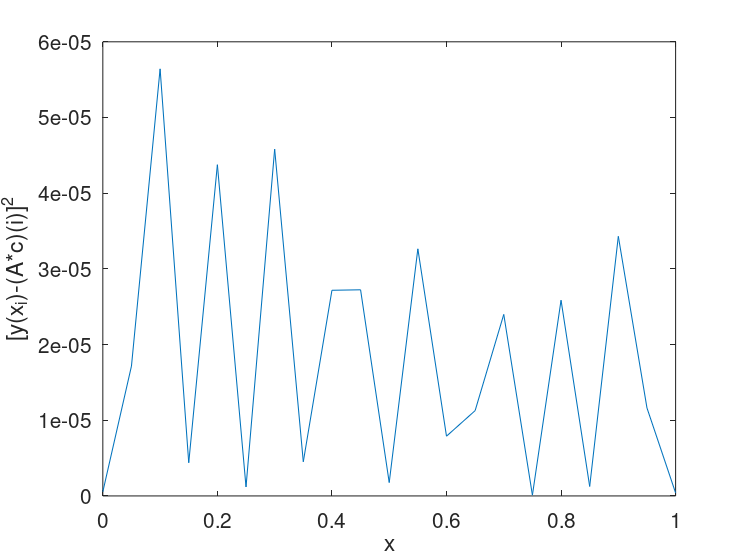
\includegraphics[width=11cm]{house}
\end{figure}
\begin{figure}[H]
\centering
\caption{\label{fig:4} Erro quadratico ponto a ponto para Cholesky}
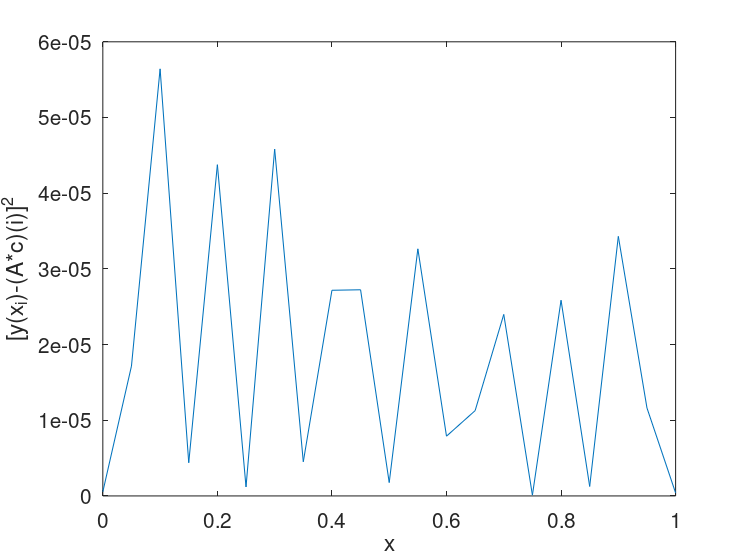
\includegraphics[width=11cm]{cholesky}
\end{figure}
\begin{figure}[H]
\centering
\caption{\label{fig:5} Erro quadratico ponto a ponto para GSM}
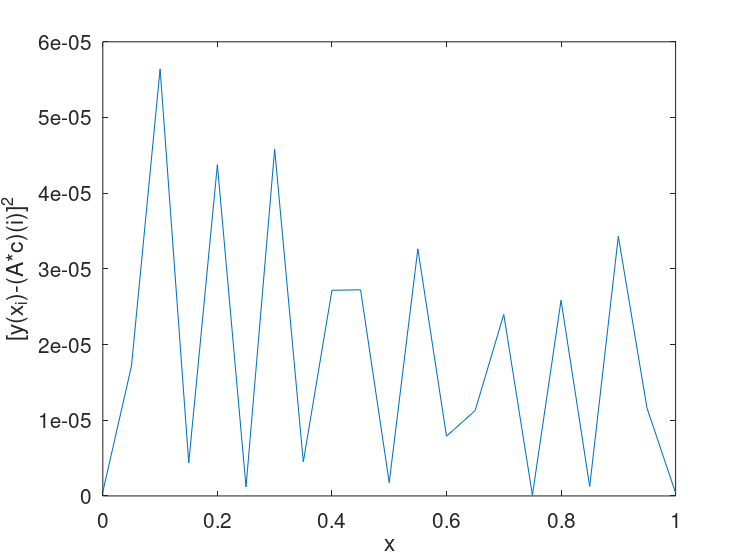
\includegraphics[width=11cm]{GSM}
\end{figure}
Código para Householder:
\begin{verbatim}
n=11;
m=21;
Xspace=linspace(0,1,m);
A=vander(Xspace);
A=A(:,n:end);
Yspace=transpose(exp(sin(6.*Xspace)));

[Q,R]=qr(A);
c=R\(Q'*Yspace);

err=(Q*R-A);
max(max(abs(err)))
err=err.^2;
MSE=sum(err(:))/numel(A)

err=(Yspace-A*c).^2;
MSE=sum(err(:))/m

plot(Xspace, err)
xlabel('x')
ylabel('[y(x_i)-(A*c)(i)]^2')
figure()

plot(Xspace, Yspace, Xspace, A*c)
xlabel('x')
ylabel('y')

cond(R)
\end{verbatim}
Código para Cholesky:
\begin{verbatim}
n=11;
m=21;
Xspace=linspace(0,1,m);
A=vander(Xspace);
A=A(:,n:end);
Yspace=transpose(exp(sin(6.*Xspace)));

ATA=A'*A; 
R=chol(ATA); 
Q=A*inv(R); 
c=R\(Q'*Yspace); 

err=(Q*R-A);
max(max(abs(err)))
err=err.^2;
MSE=sum(err(:))/numel(A)

err=(Yspace-A*c).^2;
MSE=sum(err(:))/m

plot(Xspace, err)
xlabel('x')
ylabel('[y(x_i)-(A*c)(i)]^2')
figure()

plot(Xspace, Yspace, Xspace, A*c)
xlabel('x')
ylabel('y')

cond(ATA)
cond(R)
\end{verbatim}
Código para GSM:
\begin{verbatim}
n=11;
m=21;
Xspace=linspace(0,1,m);
A=vander(Xspace);
A=A(:,n:end);
Acopia=A;
Yspace=transpose(exp(sin(6.*Xspace)));
R=zeros(n);
Q=zeros(m,n);

for j=1:n
    for i=1:j-1
        R(i,j)=Q(:,i)'*A(:,j);
        A(:,j)-=R(i,j)*Q(:,i);
    end
    R(j,j)=norm(A(:,j));
    if (R(j,j)==0)
        break
    end
    Q(:,j)=A(:,j)/R(j,j);
end
c=R\(Q'*Yspace);

err=(Q*R-Acopia);
max(max(abs(err)))
err=err.^2;
MSE=sum(err(:))/numel(A)

err=(Yspace-Acopia*c).^2;
MSE=sum(err(:))/m

plot(Xspace, err)
xlabel('x')
ylabel('[y(x_i)-(A*c)(i)]^2')
figure()

plot(Xspace, Yspace, Xspace, Acopia*c)
xlabel('x')
ylabel('y')

cond(R)
\end{verbatim}
Código para a Parte II:
\begin{verbatim}
n=9;
m=25;
Tspace=transpose(linspace(0,24,25));
A=[cos((4*pi/12).*Tspace), sin((4*pi/12).*Tspace), cos((3*pi/12).*Tspace), 
sin((3*pi/12).*Tspace), cos((2*pi/12).*Tspace), sin((2*pi/12).*Tspace), 
cos((pi/12).*Tspace), sin((pi/12).*Tspace), ones(m,1)];
Yspace=[110.49; 
73.72; 
23.39; 
17.11; 
20.31; 
29.37; 
74.74; 
117.02; 
298.04; 
348.13; 
294.75; 
253.78; 
250.48; 
239.48; 
236.52; 
245.04; 
286.74; 
304.78; 
288.76; 
247.11; 
216.73; 
185.78; 
171.19; 
171.73; 
164.05]

[Q,R]=qr(A);
c=R\(Q'*Yspace);

err=(Q*R-A);
max(max(abs(err)))
err=err.^2;
MSE=sum(err(:))/numel(A)

err=(Yspace-A*c).^2;
MSE=sum(err(:))/m

plot(Tspace, err)
xlabel('t (Horas)')
ylabel('[y(t_i)-(A*c)(i)]^2')
figure()

plot(Tspace, A*c)
hold();
scatter(Tspace, Yspace)
xlabel('t (Horas)')
ylabel(strcat('y (\mu','g/m^3)'))

cond(R)
cond(A'*A)
\end{verbatim}
\end{document}


